% Copyright 2014 David W. Hogg (NYU).  All rights reserved.

\documentclass[pdftex]{beamer}
\usepackage{amssymb,amsmath,mathrsfs}
\usecolortheme{default}

% this one is debatable
\renewcommand{\emph}[1]{\textbf{#1}}

%%% color commands
\newcommand{\whiteonblack}{%
  \colorlet{fg}{white}
  \colorlet{bg}{black}
  \setbeamercolor{normal_text}{fg=white,bg=black}
  \setbeamercolor{background canvas}{fg=white,bg=black}
  \setbeamercolor{alerted_text}{fg=yellow}
  \setbeamercolor{example_text}{fg=white}
  \setbeamercolor{structure}{fg=white}
  \setbeamercolor{palette_quaternary}{fg=white}
}
\newcommand{\blackonwhite}{%
  \colorlet{fg}{black}
  \colorlet{bg}{white}
  \setbeamercolor{normal_text}{fg=black,bg=white}
  \setbeamercolor{background canvas}{fg=black,bg=white}
  \setbeamercolor{alerted_text}{fg=blue}
  \setbeamercolor{example_text}{fg=black}
  \setbeamercolor{structure}{fg=black}
  \setbeamercolor{palette_quaternary}{fg=black}
}
\xdefinecolor{pink}{rgb}{1.0,0.9,0.9}

%%% size and shape commands
\newlength{\figurewidth}
\setlength{\figurewidth}{0.9\textwidth}
\newlength{\figureheight}
\setlength{\figureheight}{0.9\textheight}

%%% text commands
\newcommand{\project}[1]{\textsl{#1}}
  \newcommand{\an}{\project{Astrometry.net}}
  \newcommand{\tc}{\project{The~Cannon}}
  \newcommand{\euclid}{\project{Euclid}}
  \newcommand{\flickr}{\project{flickr}}
  \newcommand{\gaia}{\project{Gaia}}
  \newcommand{\galex}{\project{GALEX}}
  \newcommand{\kepler}{\project{Kepler}}
  \newcommand{\GALEX}{\galex}
  \newcommand{\hst}{\project{HST}}
  \newcommand{\hipparcos}{\project{Hipparcos}}
  \newcommand{\lsst}{\project{LSST}}
  \newcommand{\sdss}{\project{SDSS}}
  \newcommand{\sdssiii}{\project{SDSS-III}}
  \newcommand{\sdssiv}{\project{SDSS-IV}}
  \newcommand{\boss}{\sdssiii\ \project{BOSS}}
  \newcommand{\osss}{\project{OSSS}}
  \newcommand{\ska}{\project{SKA}}
  \newcommand{\vo}{\project{VO}}
  \newcommand{\rttd}{\project{Right Thing To Do}$^{\mbox{\scriptsize\sffamily{TM}}}$}
\newcommand{\foreign}[1]{\textit{#1}}
\newcommand{\latin}[1]{\foreign{#1}}
  \newcommand{\cf}{\latin{cf.}}
  \newcommand{\eg}{\latin{e.g.}}
  \newcommand{\etal}{\latin{et~al.}}
  \newcommand{\etc}{\latin{etc.}}
  \newcommand{\ie}{\latin{i.e.}}
  \newcommand{\vs}{\latin{vs.}}

%%% math-mode commands
\newcommand{\unit}[1]{\mathrm{#1}}
  \newcommand{\rad}{\unit{rad}}
  \newcommand{\s}{\unit{s}}
  \newcommand{\yr}{\unit{yr}}
  \newcommand{\km}{\unit{km}}
  \newcommand{\kmps}{\km\,\s^{-1}}
\newcommand{\mmatrix}[1]{\boldsymbol{#1}}
\newcommand{\tv}[1]{\boldsymbol{#1}}
\newcommand{\dd}{\mathrm{d}}
\newcommand{\given}{\,|\,}
\newcommand{\Teff}{T_{\mathrm{eff}}}
\newcommand{\logg}{\log g}
\newcommand{\vsini}{v\,\sin i}
 % hogg standard colors
\setlength{\paperheight}{3.5in}
% 1.77778 is the ratio of 16 to 9
% \setlength{\paperwidth}{1.77778\paperheight}
% 1.33333 is the ratio of 4 to 3
\setlength{\paperwidth}{1.33333\paperheight}
\setlength{\textwidth}{0.85\paperwidth}
\usepackage{amssymb,amsmath,mathrsfs}

\newcommand{\data}{\mbox{data}}
\newcommand{\pars}{\mbox{parameters}}

\title{Data Analysis Challenges in Astrophysics}
\author[David W. Hogg (NYU)]{David W. Hogg \\[1ex]
  \textsl{\small Center for Cosmology and Particle Physics\\
                 Department of Physics\\
                 New York University\\[2ex]
                 Center for Data Science\\
                 New York University\\[2ex]
                 Max-Planck-Institut f\"ur Astronomie\\
                 Heidelberg, Germany}}

\begin{document}

\begin{frame}
  \titlepage
\end{frame}

\begin{frame}
  \frametitle{Moore--Sloan Data Science Environments}
  \begin{itemize}
  \item Berkeley, UW, and NYU
  \item build and disseminate good practices and tools
  \item create spaces and curricula that support interdisciplinary research
  \item design and foster careers for data scientists in academia
  \end{itemize}
\end{frame}

\begin{frame}
  \frametitle{scale of data in astrophysics}
  \begin{itemize}
  \item \textsl{Sloan Digital Sky Survey}
    \begin{itemize}
    \item $10^{12}$~pixels, 5 bands per pixel
    \item $10^6$~spectra, 2000 pixels per spectrum
    \end{itemize}
  \item \textsl{Large Synoptic Survey Telescope}
    \begin{itemize}
    \item one \textsl{SDSS} per month for a decade
    \end{itemize}
  \item NASA \textsl{Kepler}
    \begin{itemize}
    \item $10^6$ images, $10^8$ pixels per image
    \item co-adds and censors data for bandwidth!
    \item (space missions are all bandwidth-limited)
    \end{itemize}
  \item \textsl{Square Kilometer Array}
    \begin{itemize}
    \item plans to throw away data in real time
    \end{itemize}
  \item all data are \emph{public} with \emph{no licensing restrictions}
  \end{itemize}
\end{frame}

\begin{frame}
  \frametitle{data science---computational definition}
  \begin{itemize}
  \item Is computation a significant issue for your data analysis?
  \end{itemize}
\end{frame}

\begin{frame}
  \frametitle{scales of The Universe}
  \begin{itemize}
  \item Earth: light-ms, days
  \item Solar System: light-min, years
  \item Galaxy: $10^4$~lyr, $10^8$~yr
  \item Universe: $10^{10}$~lyr, $10^{10}$~yr
  \end{itemize}
\end{frame}

\begin{frame}
  \frametitle{comprehensive projects}
  \begin{itemize}
  \item \emph{the Universe is big but finite}
  \item<2-> position of ``every'' galaxy and quasar out to some high redshift
  \item<2-> amplitude of ``every'' large-scale structure mode inside the visible Universe
  \item<2-> position, velocity, and chemistry of ``every'' star in the Milky Way Galaxy
  \item<2-> size, mass, and period of ``every'' planet in the Solar Neighborhood
  \item<3> of course, \emph{we only get photons}; nothing else
  \end{itemize}
\end{frame}

\begin{frame}
  \frametitle{classification in astrophysics}
  \begin{itemize}
  \item typical classification problem ``find kittehs''
    \begin{itemize}
    \item large corpus of labeled data
    \item learn flexible model on labeled data
    \item put labels on unlabeled data
    \end{itemize}
  \item requires or assumes:
    \begin{itemize}
    \item only interested in performance
    \item labels are confidently known
    \item labeled data are statistically similar to unlabeled data
    \end{itemize}
  \item<2> \emph{none of these is true} in astrophysics
  \end{itemize}
\end{frame}

\begin{frame}
  \frametitle{star--quasar classification}
  \begin{itemize}
  \item stars live in our Milky Way
  \item quasars live at the edge of the visible Universe
  \item in imaging they look \emph{incredibly} similar; stars enormously outnumbering quasars
  \item distinguishing them by spectroscopy is \emph{expensive}
  \end{itemize}
\end{frame}

\begin{frame}
\includegraphics<1>[height=\textheight]{../engineering/xdqso.png}
\end{frame}

\begin{frame}
  ~ \hfill 1-epoch \hfill model \hfill 30-epoch
  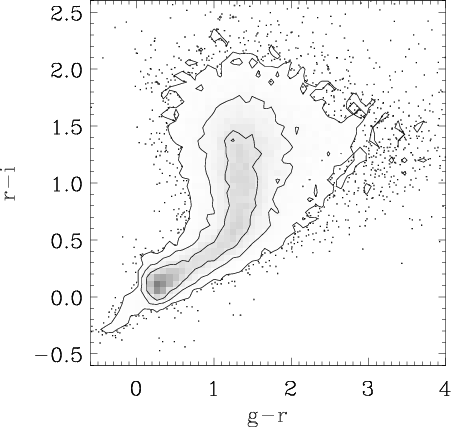
\includegraphics[width=0.35\textwidth,clip=]{../engineering/single_data_200_i_202_ri_gr.png}%
  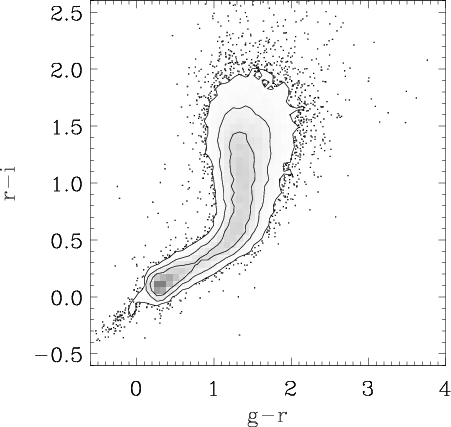
\includegraphics[width=0.35\textwidth,clip=]{../engineering/coadd_data_200_i_202_ri_gr.png}%
  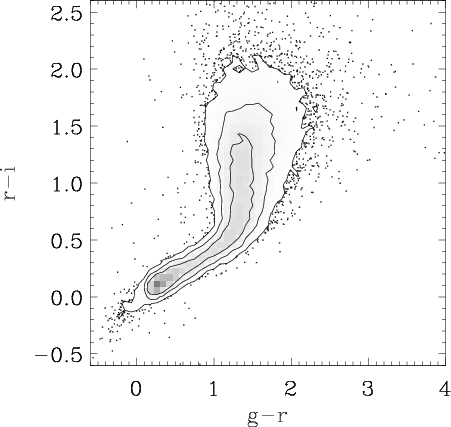
\includegraphics[width=0.35\textwidth,clip=]{../engineering/dc_fluxdist_resample_200_i_202_20_ri_gr.png}
\end{frame}

\begin{frame}
  \frametitle{physics-driven and data-driven models}
  \begin{itemize}
  \item most astrophysics problems have this form:
  \item part of the model is rigid, based on known physics
  \item the rest (majority) is ``weather'' for which we need flexible, data-driven models
    \begin{itemize}
    \item in the classification problem, the \emph{noise model} is physics driven
    \item the \emph{quasar population model} is data-driven
    \end{itemize}
  \end{itemize}
\end{frame}

\begin{frame}
  \includegraphics<1>[width=1.05\textwidth]{../engineering/p1640data.png}
  \includegraphics<2>[width=1.05\textwidth]{../engineering/p1640detections.png}
  \includegraphics<3>[width=1.05\textwidth]{../engineering/p1640method.png}
  \includegraphics<4>[width=1.05\textwidth]{../engineering/p1640spectra.png}
\end{frame}

\begin{frame}
  \frametitle{finding tiny signals---exoplanets}
  \begin{itemize}
  \item let's find an Earth analog in \textsl{Kepler} data
  \item the planet produces a \emph{tiny} imprint
    \begin{itemize}
    \item [on the board]
    \item a dip in brightness at the $10^{-4}$ level
    \item ten hours long, once per year
    \end{itemize}
  \item there are many sources of noise
    \begin{itemize}
    \item photon shot noise ($\sqrt{N}$)
    \item stochastic stellar variability
    \item issues with spacecraft calibration and stability
    \end{itemize}
  \end{itemize}
\end{frame}

\begin{frame}
  \includegraphics<1>[height=\textheight]{planet_properties.pdf}
  \includegraphics<2>[height=\textheight]{kepler-20-plm.pdf}
  \includegraphics<3>[width=\textwidth]{kic-10593626-synth.pdf}
\end{frame}

\begin{frame}
  \frametitle{finding tiny signals---cosmology}
  \begin{itemize}
  \item weak gravitational lensing in the shapes of galaxies
  \item baryonic acoustic feature in the variance of the galaxy density field
  \item B-mode polarization in the cosmic microwave background
  \end{itemize}
\end{frame}

\begin{frame}
  \frametitle{map--reduce or die}
  \begin{itemize}
  \item \textsl{``We won't even consider algorithms that can't be
    written in the map--reduce framework.''}
    \begin{itemize}
    \item (Kai Li spoke to this)
    \end{itemize}
  \end{itemize}
\end{frame}

\begin{frame}
  \frametitle{map--reduce}
  \includegraphics[width=1.1\textwidth]{../../pgm/mapreduce.pdf}
\end{frame}

\begin{frame}
  \frametitle{map--reduce and computational scalings}
  \begin{itemize}
  \item You can evaluate a likelihood or a gradient in map--reduce framework.
  \item You \emph{can't} do probabilistic inference in map--reduce.
  \item New computational frameworks will create new opportunities!
  \end{itemize}
\end{frame}

\begin{frame}
  \frametitle{imaging challenges}
  \begin{itemize}
  \item coronography
  \item radio interferometry
  \item probabilistic models for images
  \end{itemize}
\end{frame}

\begin{frame}
  \frametitle{living the likelihood dream}
  \begin{itemize}
  \item Astronomers love catalogs (unfortunately).
    \begin{itemize}
    \item that's some kind of (very inefficient) estimator
    \item even with error bars it can't transmit the full information
    \end{itemize}
  \item produce a likelihood function in \emph{catalog space}
    \begin{itemize}
    \item Lang \etal\ \url{http://TheTractor.org/}
    \item Brewer \etal\ arXiv:1211.5805
    \item inferences with thousands to \emph{billions} of parameters
    \end{itemize}
  \end{itemize}
\end{frame}

\begin{frame}
  \includegraphics<1>[width=1.05\textwidth]{brewer1.png}
  \includegraphics<2>[height=\textheight]{brewer2.png}
  \includegraphics<3>[width=1.05\textwidth]{brewer3.png}
  \includegraphics<4>[width=\textwidth]{../../pgm/crowded.png}
\end{frame}

\begin{frame}
  \frametitle{spectroscopy challenges}
  \begin{itemize}
  \item all the imaging challenges, plus:
  \item unknown atomic and molecular physics
  \end{itemize}
\end{frame}

\begin{frame}
  \frametitle{summary}
  \begin{itemize}
  \item achievable comprehensive data-taking goals
  \item large data sets
  \item tiny signals
  \item probabilistic forward modeling
  \item mixtures of physics-driven and data-driven models
  \end{itemize}
\end{frame}

\end{document}

\begin{frame}
  \frametitle{fubar}
  \begin{itemize}
  \item foo
  \item foo
    \begin{itemize}
    \item bar
    \item bar
    \end{itemize}
  \item foo
  \end{itemize}
\end{frame}

